\section{Literature Review} \label{sec:literature}

This section is divided into three parts. Section \ref{sec:ensinointegral} reviews the literature on full-time schooling programs, particularly in the Brazilian and South American contexts. Section \ref{sec:peisaopaulo} describes the PEI in the state of São Paulo, detailing its staggered implementation and discussing recent findings on student composition. Finally, Section \ref{sec:diffindiff} discusses the evolution of difference-in-differences estimators and motivates the methodological choices in this paper.

%-----------------------------------------------------------------------
\subsection{Full-Time Education} \label{sec:ensinointegral}
%-----------------------------------------------------------------------

Increasing instructional time is often cited as a central lever for improving educational quality. One of the first papers to address this subject in the South American context is \textcite{bellei2009}, which evaluated a full-time school program in Chile. Using a Difference-in-Differences methodology, the author found positive and heterogeneous effects, with the program generating a greater impact in rural areas, among public school students, and students already at the top of the performance distribution.

In the Brazilian context, however, the literature demonstrates that results vary drastically depending on the design and depth of the educational policy adopted. \textcite{AlmeidaEtAl2016MaisEducacao} evaluated the federal program \textit{"Mais Educação"}, which focused on providing complementary extracurricular activities, increasing the daily school load to a minimum of 7 hours. Despite the extra funding, the authors found a null impact on standardized test scores in Portuguese and on school dropout rates, and even a negative impact on Mathematics. This result suggests that simple extension of school hours, without profound pedagogical restructuring, is insufficient to leverage learning.

On the other hand, more structured state programs have shown success. In Pernambuco, \textcite{Pernambuco} found significant gains in Mathematics and Language (approximately 0.22 and 0.19 standard deviations) resulting from the state full-time education program. Complementarily, \textcite{araujo2020_pernambuco_impacto_enem} showed that this same program positively affected scores on the National High School Exam (ENEM), highlighting a "multiplier effect" of hours spent on complementary activities.

In the State of São Paulo, the precursor experience of the \textit{"Programa Escola de Tempo Integral"} (ETI), implemented between 2007 and 2008, illustrates the difficulties of school day extension policies. \textcite{aquino2011_eti_2007_2008_psm_painel} analyzed the ETI using panel data and Propensity Score Matching, finding essentially null results in Mathematics and passing rates. The author points out that the lack of activity planning focused on proficiency and coordination problems motivated the initiative's failure. It is evident, therefore, that there was a need for a program that combined classroom time with a new management and teaching architecture gap that would later be filled by the PEI.

%-----------------------------------------------------------------------
\subsection{The Integral Education Program (PEI) in São Paulo} \label{sec:peisaopaulo}
%-----------------------------------------------------------------------

Established in 2012, the Integral Education Program (PEI) emerged as the main bet of the São Paulo state network to overcome the bottlenecks of previous models. The formulation of the PEI distinguishes itself by proposing a full-time school that combines extended stay (8 to 9 hours daily) with a profound redesign of the pedagogical project and the management model \parencite{sao_paulo_pei_2012}.

To operationalize this proposal, converted schools adopted innovations such as the \textit{Life Project} (where students structure their long-term goals), Electives, Experimental Practices, and Tutoring. From a management perspective, the program introduced the PDCA (Plan, Do, Check, and Act) methodology and established the Full and Integral Dedication Regime (RDPI), which guarantees a 75\% salary bonus for teachers and managers in exchange for exclusive dedication to a single school unit, preventing the faculty from splitting their time between multiple schools \parencite{sao_paulo_pei_2012}. The implementation of the PEI occurred in a non-random and staggered manner over time. As illustrated in Figure \ref{fig:rolloutnovas}, the program began with a restricted group of schools in 2012, increasing substantially over the years.

\begin{figure}[htbp]
\centering
\caption{New PEI schools by year of adoption}
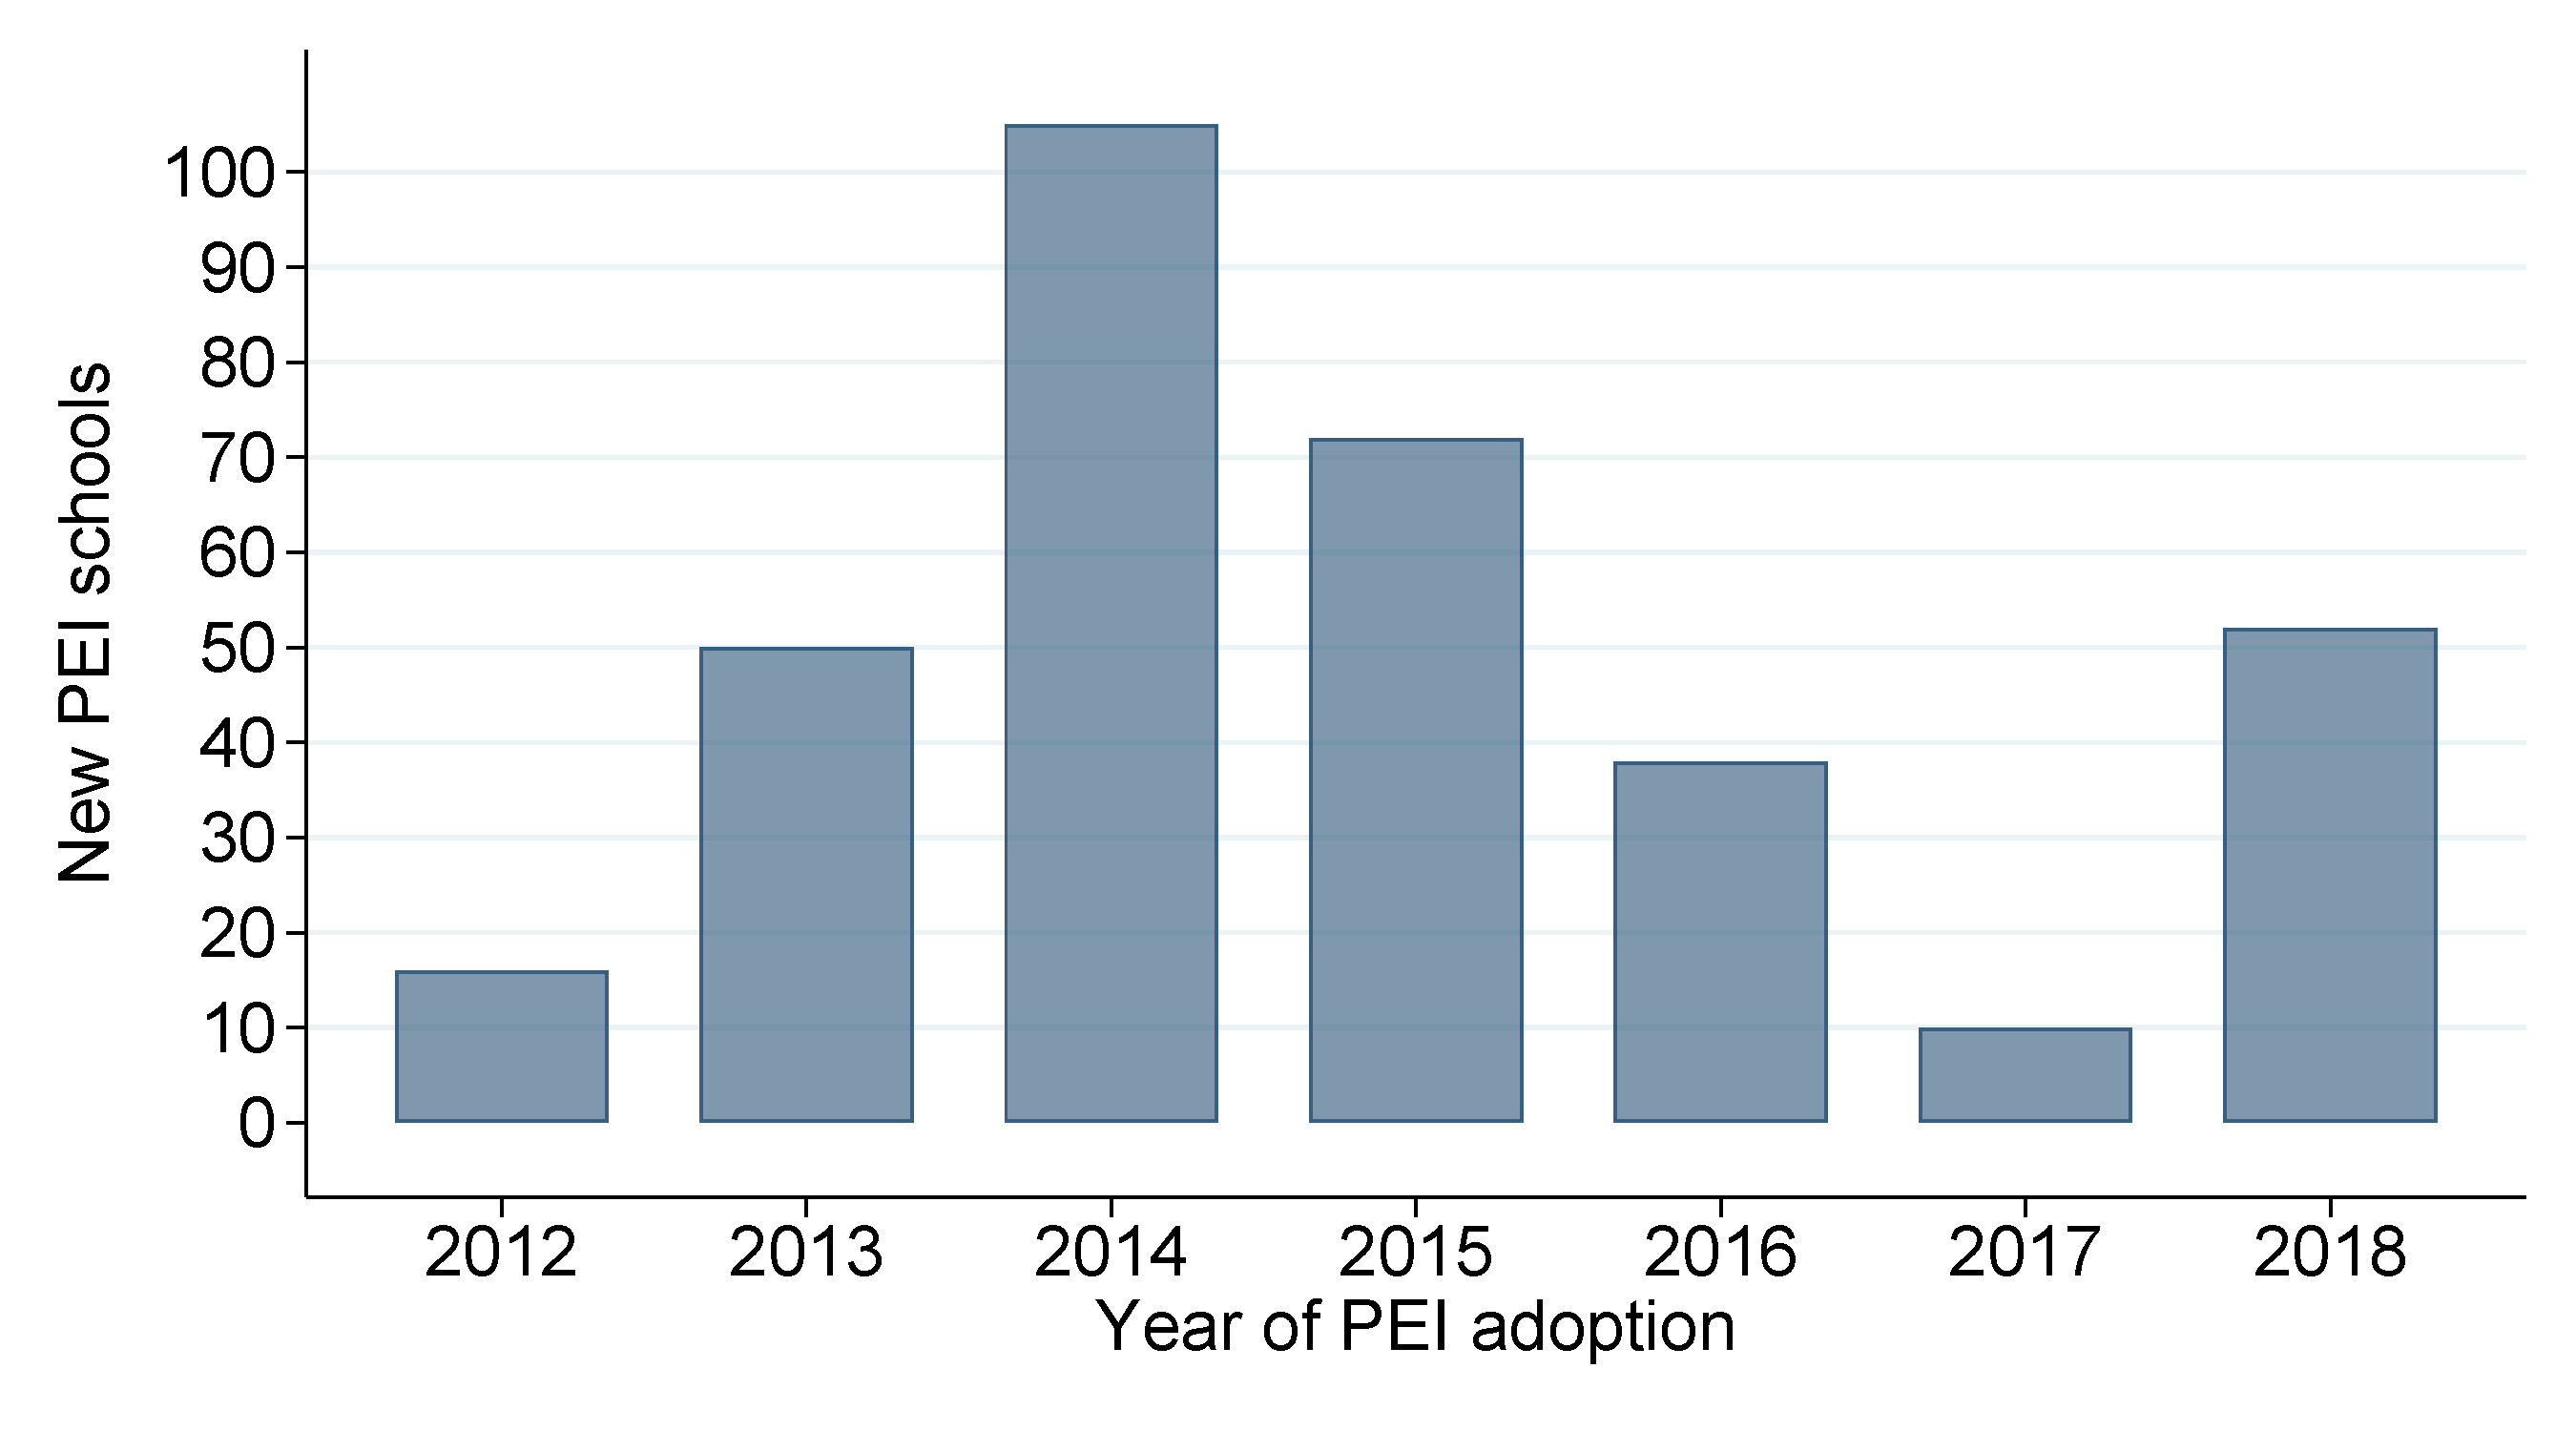
\includegraphics[width=0.7\textwidth]{files/images/rollout_novas.pdf}
\label{fig:rolloutnovas}
\caption*{\footnotesize \textit{Source:} \href{https://dados.educacao.sp.gov.br/story/saresp}{SP Education Open Data}. Author's elaboration.}
\end{figure}

Figure \ref{fig:rolloutacumulado} highlights the magnitude of this rollout, showing the consolidation of the PEI as a large-scale policy in the São Paulo educational system. Conditional adherence based on infrastructure criteria in the early years reinforces the character of the PEI as a change in a complex institutional arrangement, rather than a mere exogenous time shock.

\begin{figure}[htbp]
\centering
\caption{Cumulative number of PEI schools in the state of São Paulo}
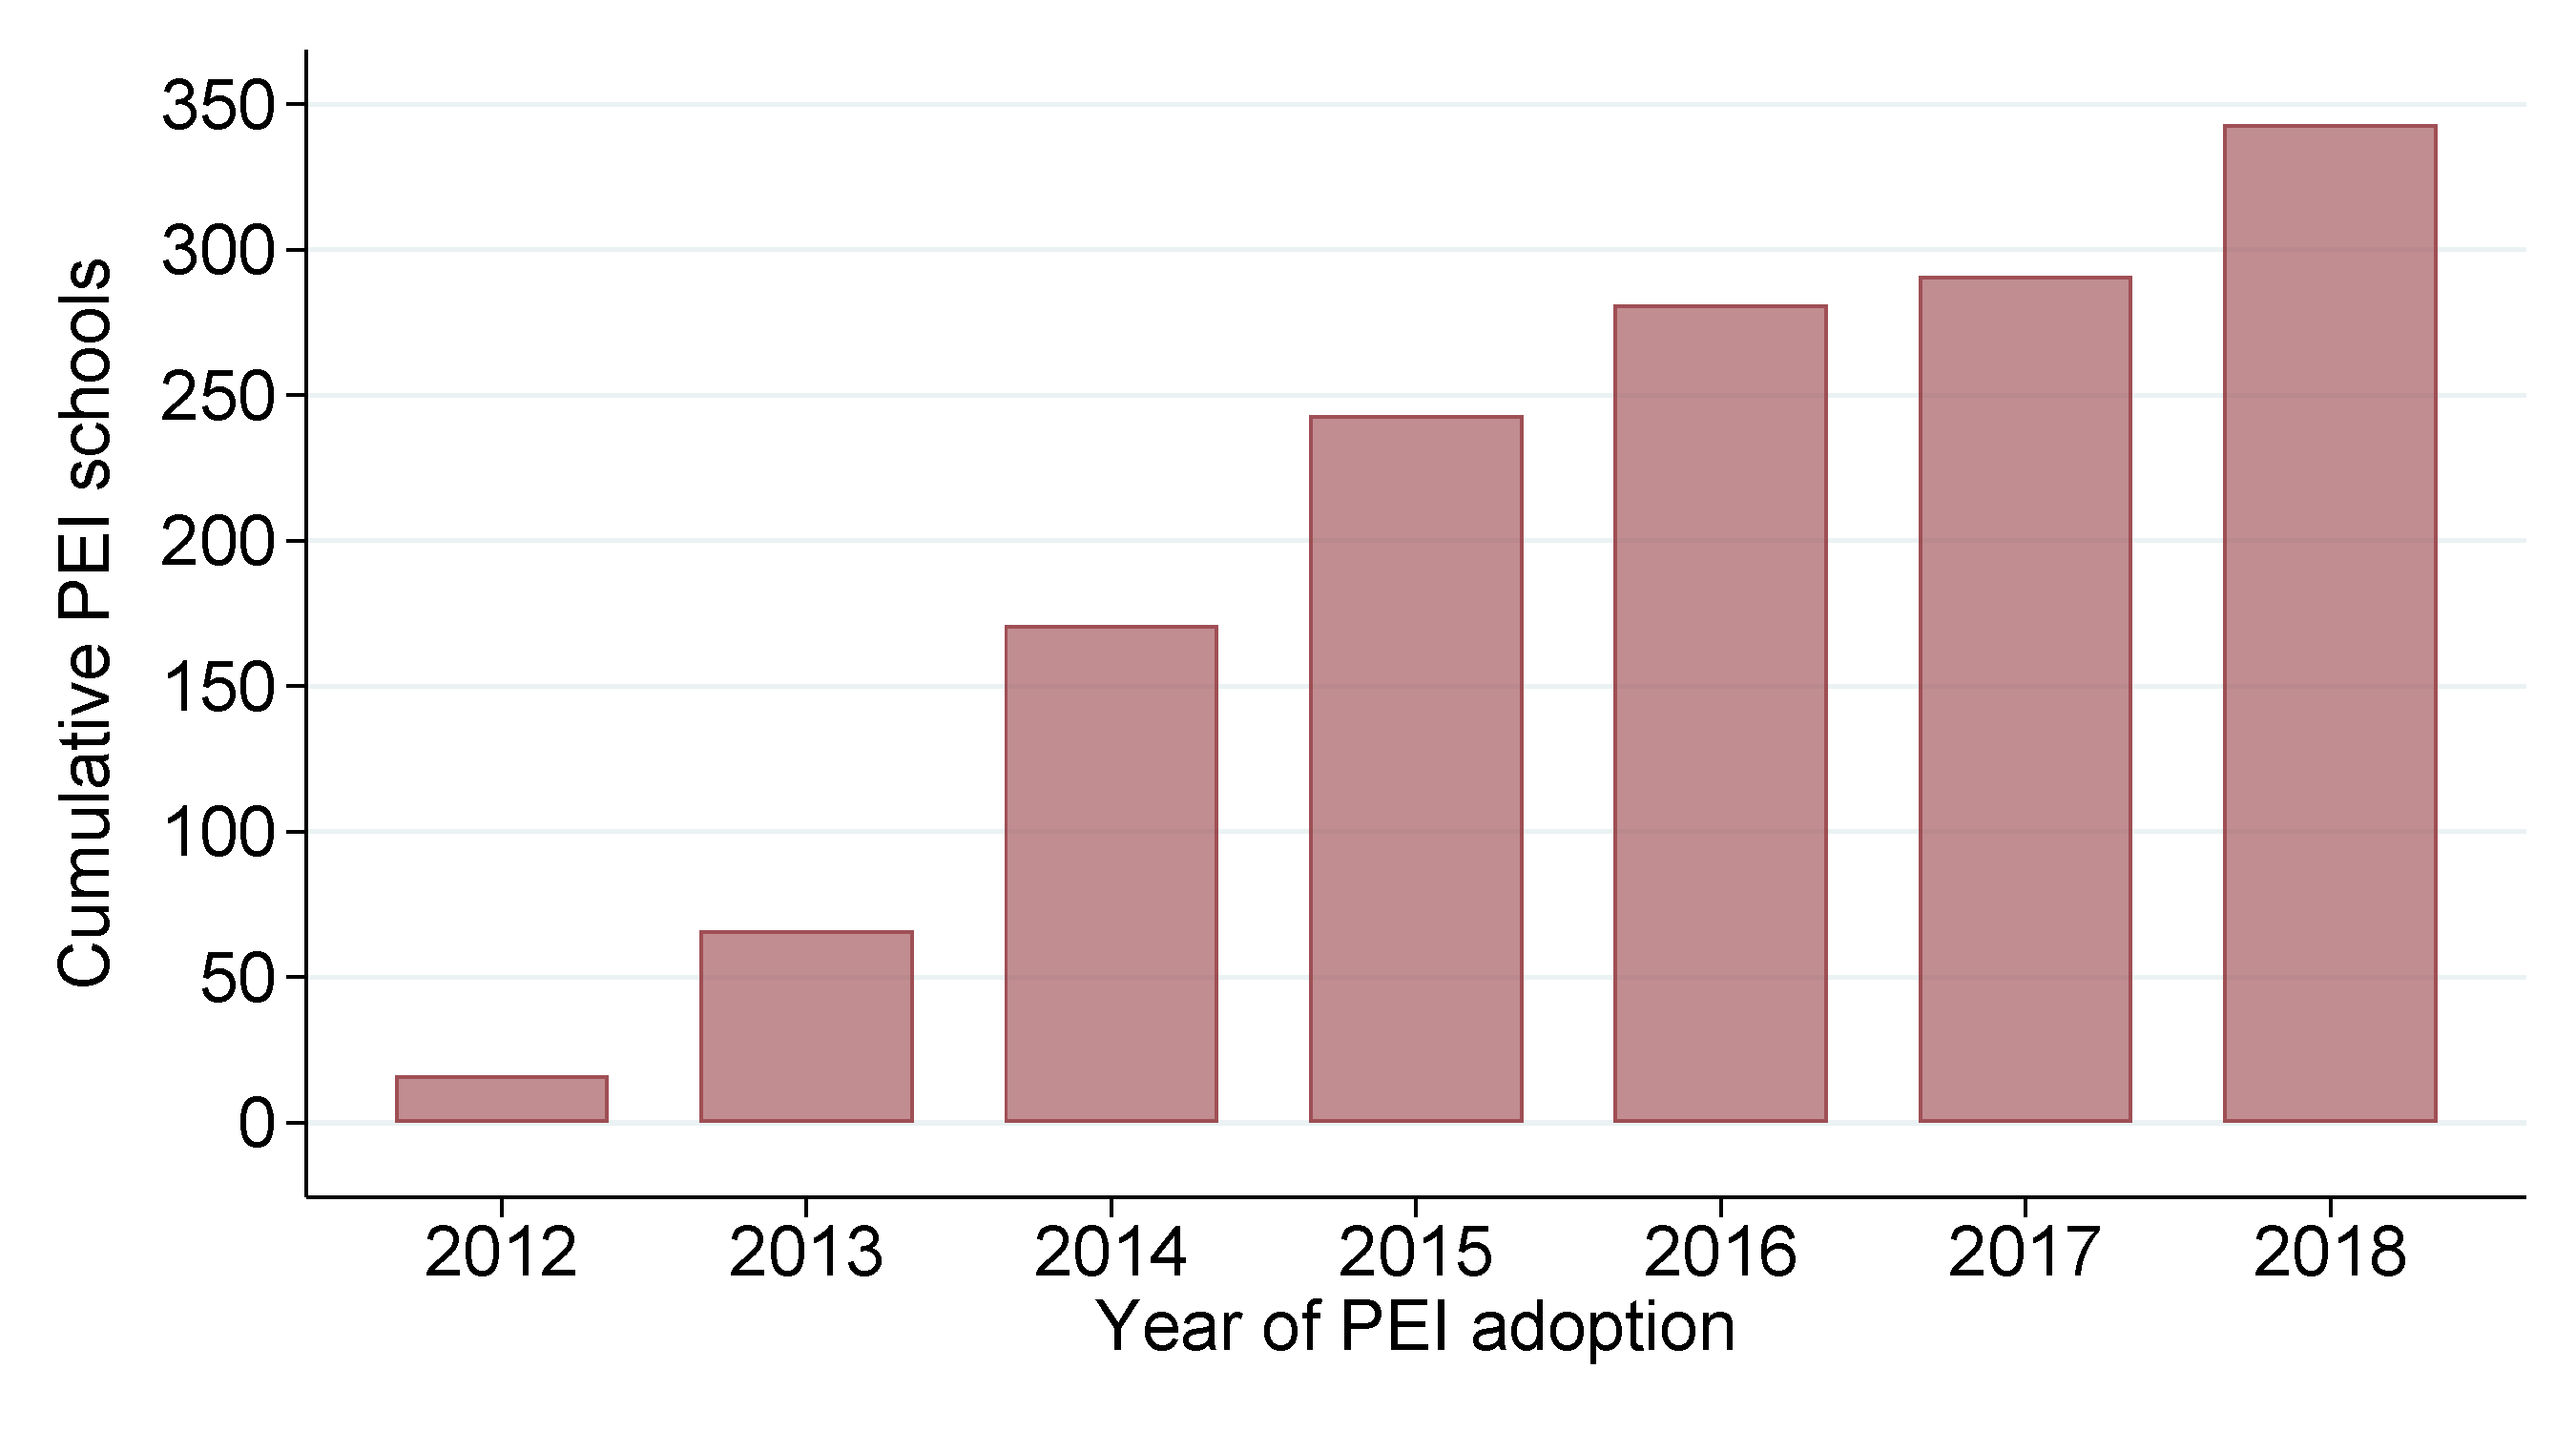
\includegraphics[width=0.7\textwidth]{files/images/rollout_acumulado.pdf}
\label{fig:rolloutacumulado}
\caption*{\footnotesize \textit{Source:} \href{https://dados.educacao.sp.gov.br/story/saresp}{SP Education Open Data}. Author's elaboration.}
\end{figure}

Early empirical evaluations of the PEI attest to its success in raising human capital. \textcite{pei_saeb} applied Difference-in-Differences to estimate the impact on SAEB results, reporting gains of about 0.46 standard deviations in Mathematics and Portuguese. Additionally, \textcite{kawahara2019_pei_impacto_enem_provabrasil_fluxo} found positive impacts on ENEM performance, \textit{Prova Brasil} (a biennial assessment applied to students in public schools), and school flow indicators. More recently, \textcite{scorzafave2023} directly evaluated the impact on SARESP High School scores, finding gains of 0.31 and 0.21 standard deviations in Mathematics and Portuguese, respectively.

Despite the strong consensus surrounding positive direct results, a recent and critical literature has raised structural concerns regarding how the program affects the state network. \textcite{favaro_composicao_pei} analyzed compositional changes associated with program adoption and documented that the conversion to PEI actively alters the profile of the student body: the program increased the fraction of girls and reduced the percentage of non-white students and students with school age-grade distortion. Furthermore, a reduction in the total number of enrollments in newly converted schools was identified.

Simultaneously, \textcite{santos2022_spillover_pei_escolas_regulares} documented the existence of spillover effects on regular schools in the vicinity of PEI schools, showing that student migration alters the composition of neighboring schools, harming their performance. These two empirical findings—compositional change in treated units and contagion in the control group—form the basis of the problem that this work aims to solve, requiring a transition to the frontier of causal inference econometrics.

%-----------------------------------------------------------------------
\subsection{Methodological Evolution: The Evolution of Difference-in-Differences Estimators} \label{sec:diffindiff}
%-----------------------------------------------------------------------

Impact evaluation of public policies has gained centrality in contemporary economic research. As documented by \textcite{currie2020}, the discipline underwent an empirical turn in recent decades: applied microeconomics became a growing share of top journals, and quasi-experimental methods, especially difference-in-differences, came to organize a large share of causal evidence in public policy.

Despite this popularity, evaluations of public policies with multiple periods, such as the PEI rollout, historically relied almost exclusively on TWFE estimators. A recent econometric literature shows that this estimator can fail severely when the policy is adopted in a staggered manner and treatment effects are heterogeneous over time.

\textcite{goodmanbacon} shows that TWFE can make ``forbidden comparisons,'' using units already treated in earlier periods as controls for units treated later. Complementarily, \textcite{chaisemartin2020} show that this contamination may generate strictly negative aggregation weights, potentially producing estimates with the opposite sign of the true policy effect.

To address the limitations of the classical model, the literature developed new estimators. The approach of \textcite{callawaysantanna} became a primary solution for staggered adoption, isolating clean comparisons that use only not-yet-treated or never-treated units. In addition, \textcite{santannazhao} advanced doubly robust estimators that combine regression adjustment and weighting (IPW) to handle covariates efficiently.

Finally, the data structure of educational assessments imposes an additional identification challenge. Exams such as SARESP form repeated cross-sections. The concern with DiD under compositional change appears early in \textcite{hong2013}, who shows in another empirical context that the composition of observed groups may change over time and bias conventional estimators. \textcite{murto2024} revisits this argument and shows that propensity-score reweighting strategies can be adapted to handle compositional shifts in repeated cross-sections in a simpler way. As \textcite{santannaxu} emphasize, DiD estimators for this type of data usually rely on a stationarity assumption: the distribution of observed individuals in treated and control units should not change differentially because of treatment.

As \textcite{favaro_composicao_pei} documents for PEI, program adoption changes the composition of the student body in a statistically significant way. When this premise is violated by the policy itself, estimators that do not correct for composition may confuse student selection with learning gains, in addition to migration across schools. This paper starts from that concern, but adapts it to the publicly available data: instead of fully applying the individual-level estimator of \textcite{santannaxu}, I use composition covariates aggregated by school, year, and grade to evaluate the sensitivity of the estimates to observable changes in the student body.
